% ------------------------------------------------------------------------- //
% Facultad de Ingeniería de la Universidad de Buenos Aires
% Algoritmos y Programación II
% 1er Cuatrimestre de 2015
% Trabajo Práctico 1: Recursividad
% Cálculo de DFT
% 
% informe_tp1.tex
% Informe
%
% Para compilar:
% $: pdflatex informe_tp1
% ------------------------------------------------------------------------- //

% ---- Preamble ----
\documentclass{article}


% ---- Packages ----
\usepackage{amsmath} % Advanced math typesetting
\usepackage[utf8]{inputenc} % Unicode support (Umlauts etc.)
\usepackage[spanish]{babel} % Change hyphenation rules
\usepackage{hyperref} % Add a link to your document
\usepackage{graphicx} % Add pictures to your document
\usepackage{float} % For 'H' figure position option. Stricter than 'h!'
%\usepackage{listings} % Source code formatting and highlighting
\usepackage{listingsutf8} % Source code formatting and highlighting in UTF-8
\usepackage[a4paper]{geometry} % Page size options
  \geometry{tmargin=3cm,bmargin=3cm,lmargin=2cm,rmargin=2cm} % Margins
\usepackage{fancyhdr} % Add head­ers and foot­ers
  \setlength{\headheight}{14pt} % Needs to be 13.6pt or more
  \pagestyle{fancy}
  %\fancyhf{} % Clear the default settings
  %\lhead{left header content}
  %\chead{middle header content}
  %\rhead{right header content}
  %\lfoot{left footer content}
  %\cfoot{middle footer content}
  %\rfoot{right footer content}
\usepackage{color} % Colours
  %red, green, blue, yellow, cyan, magenta, black, white
  \definecolor{mygreen}{RGB}{28,172,0} % color values Red, Green, Blue
  \definecolor{mylilas}{RGB}{170,55,241}
  \definecolor{mygray}{rgb}{0.5,0.5,0.5}
  \definecolor{mymauve}{rgb}{0.58,0,0.82}
  \definecolor{myblue}{rgb}{0.33,0.33,0.99}
\hypersetup{ % Remove hyperlink borders
  pdfborder={0 0 0}
}
% ------------------

% ---- Formato para código fuente ----
\lstset{
    language=C++,
    basicstyle=\color{red},
    breaklines=true,%
    morekeywords={matlab2tikz},
    keywordstyle=\color{blue},%
    morekeywords=[2]{1}, keywordstyle=[2]{\color{green}},
    identifierstyle=\color{black},%
    stringstyle=\color{mygreen},
    commentstyle=\color{mygray},%
    showstringspaces=false,%without this there will be a symbol in the places where there is a space
    numbers=left,%
    numberstyle={\tiny \color{mygray}},% size of the numbers
    numbersep=9pt, % this defines how far the numbers are from the text
    emph=[1]{for,end,break},emphstyle=[1]\color{blue}, %some words to emphasise
    emph=[2]{word1,word2}, emphstyle=[2]{style},    
    inputencoding=utf8/latin1, % Para código con tildes y otros caracteres
}
% ------------------------------------


% --------------------------------------------------------------------------- %
% ---- Comienzo del documento ----
\begin{document}

% ---- Carátula ----
\title{Algoritmos y Programación II\\
       TP1: Recursividad}
\author{Bourbon, Rodrigo\\
        Carreño Romano, Carlos Germán\\
        Sampayo, Sebastián Lucas}
\date{Primer Cuatrimestre de 2015}
\maketitle

\begin{center}
  
\includegraphics[width=0.5\paperwidth]{Imagenes/logo_fiuba_HD}
  %\rule[depth]{width}{height}
  \rule[0.5ex]{0.8\paperwidth}{0.1pt}
\par
\end{center}

\pagenumbering{gobble} % Don't number this page
% ------------------

% ---- Encabezado ----
\lhead{Algoritmos y Programación II - TP1 - FIUBA}
% --------------------

% ---- Tabla de contenidos ----
\newpage{}
\vfill{}
\tableofcontents{}
\vfill{}
\newpage{}
% -----------------------------
% ------------------------------------
\pagenumbering{arabic} % Do number this page, arabic numbers


\section{Objetivos}
  Ejercitar técnicas de diseño, análisis, e implementación de algoritmos recursivos.

\section{Introducción}
  Explicar un poco que es la FT, la DFT y la FFT.

\section{Desarrollo}

  \subsection{Standard de estilo}
    Adoptamos la convención de estilo de código de Google para C++, salvando las siguientes excepciones:
    \begin{itemize}
      \item Streams: utilizamos flujos de entrada y salida
      \item Sobrecarga de operadores
    \end{itemize}
    \url{https://google-styleguide.googlecode.com/svn/trunk/cppguide.html#Naming}

  \subsection{Diseño del programa}
    Explicar a grandes rasgos como funciona el programa, diagrama en bloques.
    -> Leer de la entrada a vector, rellenar con ceros, transformar, imprimir vector.

  \subsection{Opciones del programa}
    El programa se ejecuta en línea de comandos, y las opciones que admite (sin importar el orden de aparición) son las siguientes:
    \begin{itemize}
      \item[] \textit{nombre largo} (\textit{nombre corto}): \textit{descripción}
      \item \texttt{--input} (\texttt{-i}): 
      \item \texttt{--output} (\texttt{-o}):
      \item \texttt{--method} (\texttt{-m}):
    \end{itemize}

  \subsection{Métodos de la Transformada}
    como fue implementado dft y fft, funciones genéricas, máscaras, complejidad temporal, espacial, etc.

  \subsection{Estructura de archivos}

  \subsection{Compilación}
  Como se compila

  \subsection{Casos de prueba}
  los q aparecen en la especificación del tp, mostrar capturas de pantalla
  de la consola ejecutando todo

\section{Código}

% Plantilla de figura:
%  \begin{figure}[H]
%  \begin{centering}
%  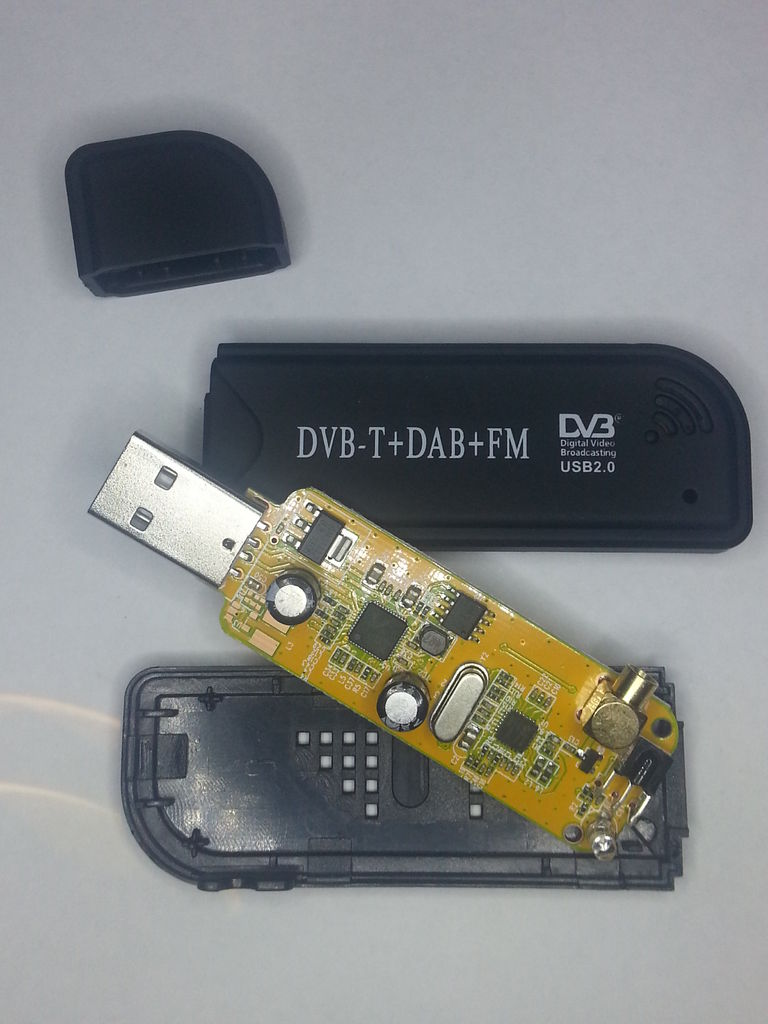
\includegraphics[width=0.75\textwidth]{Imagenes/SDR.jpg}
%  \par\end{centering}
%  \caption{Sintonizador de radio digital.}
%  \end{figure}

% Plantilla de código fuente:
%    \lstinputlisting{code.cc}

\section{Enunciado}

\end{document}
